\def\titulo{Evaluación diagnóstica}
\def\subtitulo{Números y álgebra}
\def\curso{Tercero medio}

\documentclass[sin curso]{srs}

\begin{document}

\section{Objetivo}

La siguiente evaluación tiene como objetivo medir el dominio de contenidos y habilidades
de cada estudiante, para poder diseñar un plan de estudio acorde de las necesidades del
grupo curso.

Particularmente, se medirá:
\begin{itemize}[nosep]
  \item Propiedades aritméticas de potencias, raíces y logaritmos.
  \item Solucionar ecuaciones cuadráticas.
  \item Plantear y resolver problemáticas usando lenguaje algebraico.
\end{itemize}

La nota es solo referencial y no afecta el promedio del estudiante de ninguna manera. Cada
pregunta tiene un punto.

\section{Operatoria de números}

Determine el valor de cada una de las siguientes expresiones.
\begin{preguntas}
  \pregunta $\left(\dfrac{2^2\cdot 3^5\cdot 4^2}{2^4\cdot 3^2}\right)^2 =$
  \begin{malla}[height=6cm]
  \end{malla}
  \pregunta $\left(\dfrac{7^{-1}}{2^{-1}+3^{-1}+6^{-1}}\right)^{-2} =$
  \begin{malla}[height=6cm]
  \end{malla}
  \pregunta $\sqrt[5]{2^{10}\cdot 5^{10}} =$
  \begin{malla}[height=6cm]
  \end{malla}
  \pregunta $\sqrt{\sqrt[4]{256}} =$
  \begin{malla}[height=6cm]
  \end{malla}
  \pregunta Si $log(5) = 0,69$ y $log(7)=0,84$, encontrar el valor de $log(35)$.
  \begin{malla}[height=6cm]
  \end{malla}
  \pregunta Halla el resultado de $log(\sqrt{2,5})$ si $log(2)=0,30$ y $log(5)=0,69$.
  \begin{malla}[height=6cm]
  \end{malla}
\end{preguntas}

\section{Álgebra}
Encuentre las soluciones de cada ecuación.
\begin{preguntas}
  \pregunta $x^2-5x+6=6x-18$
  \begin{malla}[height=5cm]
  \end{malla}
  \pregunta $3y^2-18=0$
  \begin{malla}[height=5cm]
  \end{malla}
  \pregunta $(y+4)^2 = 36$
  \begin{malla}[height=5cm]
  \end{malla}
\end{preguntas}

Plantee y resuelva las siguientes problemáticas.
\begin{preguntas}
  \pregunta Los físicos han encontrado que un objeto que se lanza verticalmente hacia
  arriba con una rapidez de $v_0$ [m/s] alcanzará una altura de $h=-16t^2+v_0\cdot t$ metros,
  después de $t$ segundos. \par

  Supón que una pelota se lanza hacia arriba, con una rapidez inicial de $256$ [m/s].
  ¿Qué altura máxima alcanzará la pelota?
  \begin{malla}[height=8cm]
  \end{malla}
  \pregunta Un vástago de bambú de 3 metros de largo se rompe de forma tal que su
  punta toca el suelo a 1 metro de la base, como se muestra en la figura. ¿Cuál es
  la altura a la que se rompió el vástago?
\begin{center}
    \vspace*{5mm}
    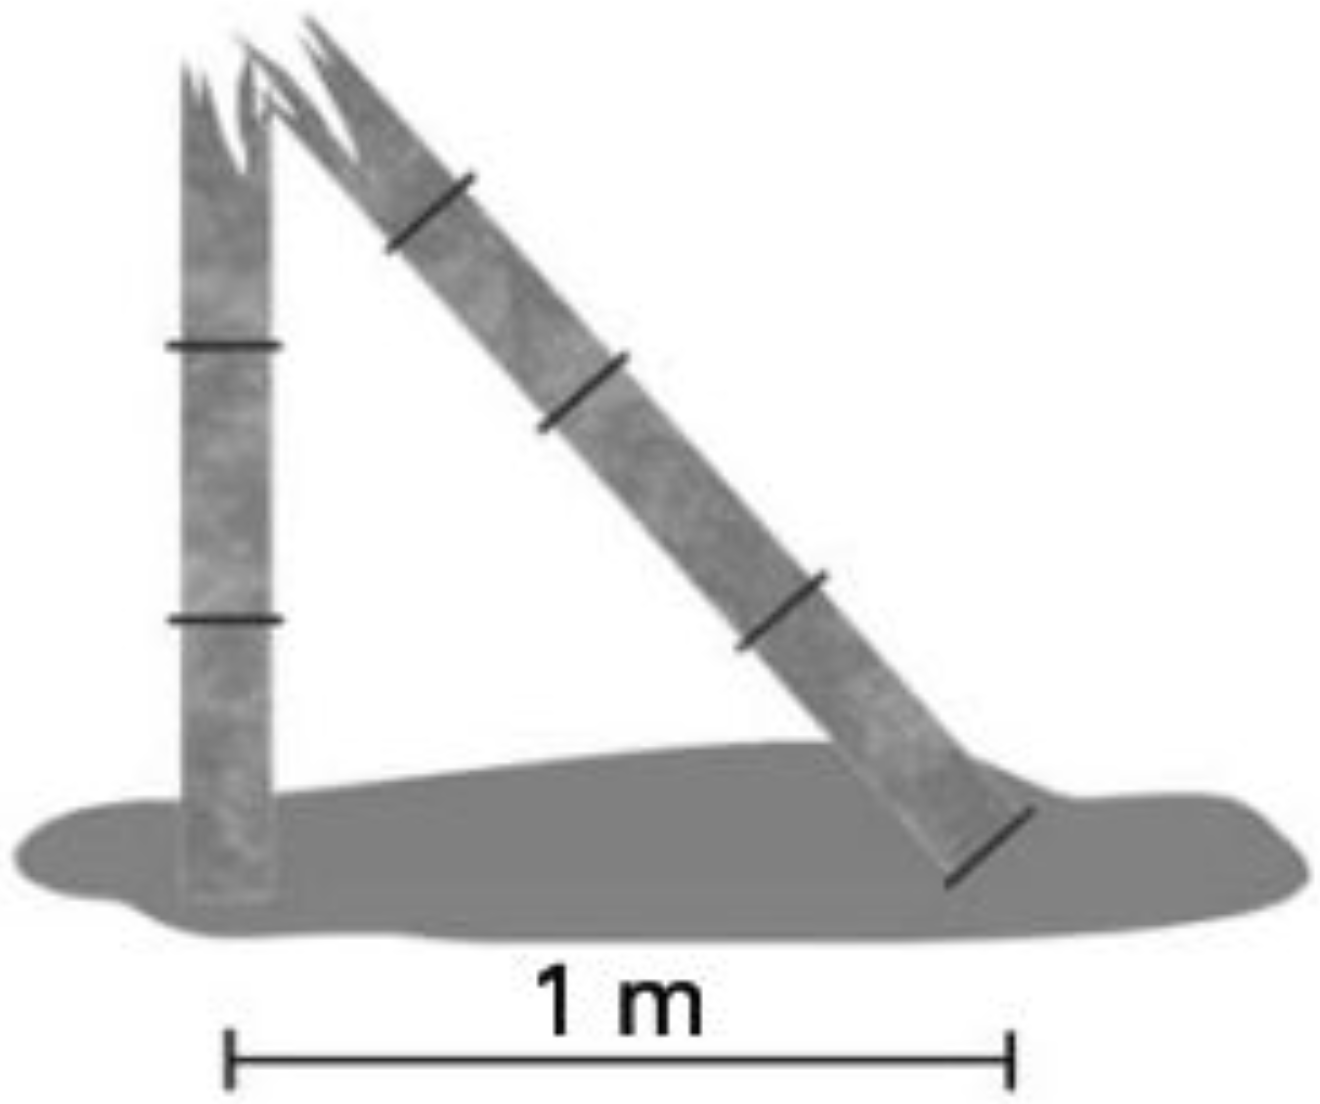
\includegraphics[width=4cm]{vastago.png}
    \vspace*{5mm}
  \end{center}
  \begin{malla}[height=8cm]
  \end{malla}
\end{preguntas}

\section{Desafíos}
\begin{preguntas}
  \pregunta Hallar el valor numérico de: $x^{\displaystyle x^{\displaystyle 1+2x^{\displaystyle 1+x-x^{\displaystyle x+1}}}}$, siendo $x^x = 2$
  \begin{malla}[height=11.5cm]
  \end{malla}
  \pregunta Halle la raíz de la ecuación: $\dfrac{1}{(x-1)^2} -\dfrac{3}{2x-2} -\dfrac{3}{2x+2} = 0$
  \begin{malla}[height=11.5cm]
  \end{malla}

\end{preguntas}
\end{document}